% To familiarize yourself with this template, the body contains
% some examples of its use.  Look them over.  Then you can
% run LaTeX on this file.  After you have LaTeXed this file then
% you can look over the result either by printing it out with
% dvips or using xdvi.
%

\documentclass[twoside]{article}
%\usepackage{soul}
\usepackage{./lecnotes_macros}


\begin{document}
%FILL IN THE RIGHT INFO.
%\lecture{**LECTURE-NUMBER**}{**DATE**}{**LECTURERS**}{**SCRIBE**}
\lecture{3}{22 January 2025}{Maria Francis and M. V. Panduranga Rao}{Gautam Singh}
%\footnotetext{These notes are partially based on those of Nigel Mansell.}

%All figures are to be placed in a separate folder named ``images''

% **** YOUR NOTES GO HERE:

\section{Cryptanalysis of DES Reduced to 8 Rounds}
DES reduced to 8 rounds uses a 5-round characteristic with probability 
approximately \(\frac{1}{10486}\) as shown in \autoref{fig:des-8-char}.

\begin{figure}[!ht]
    \centering
    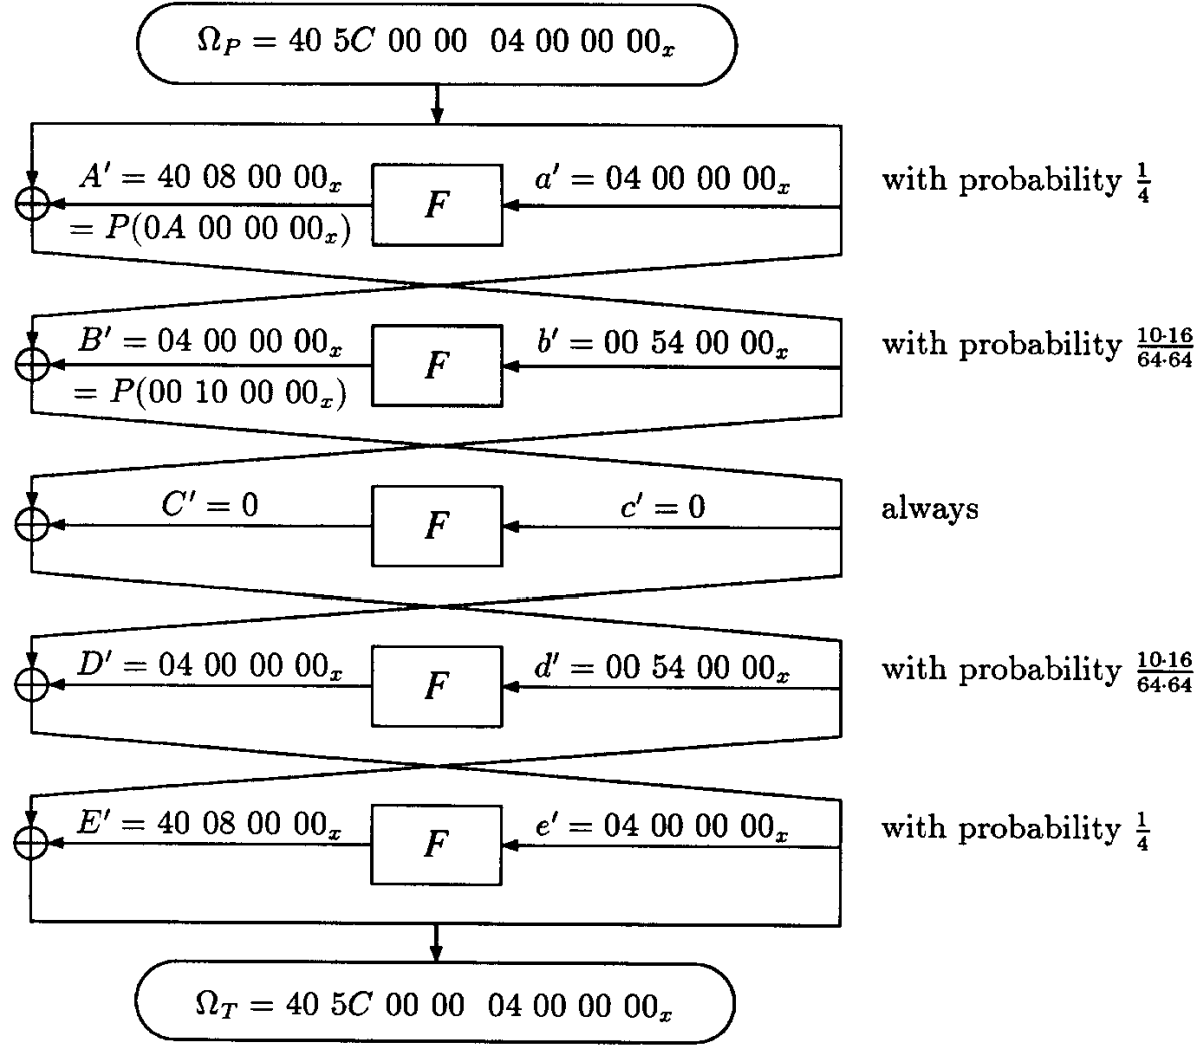
\includegraphics[width=0.5\textwidth]{images/des_8round_char.png}
    \caption{5 round characteristic used to cryptanalyze DES reduced to 8 rounds.}
    \label{fig:des-8-char}
\end{figure}

From the characteristic, it is evident that
\begin{equation}
    f^\prime = d^\prime \oplus E^\prime = b^\prime \oplus A^\prime = L^\prime = \texttt{40 5C 00 00}.
\end{equation}

Thus, for a right pair, five S boxes S2, S5, \dots, S8 have zero input XORs in
the sixth round. Using
\begin{equation}
    H^\prime = l^\prime \oplus g^\prime = l^\prime \oplus e^\prime \oplus F^\prime
\end{equation}

and the fact that \(h^\prime = r^\prime\), we can count on \(5 \cdot 6 = 30\)
key bits of \(K8\). The signal to noise ratio is \(S/N = \frac{2^{30}}{4^5 \cdot
10486} \approx 100\). However, due to the large memory requirement of \(2^{30}\)
locations, we count on fewer key bits. Further, due to the small probability of
the characteristic, we require many plaintexts, which makes the clique method
slow. Notice that each S box discards 20 \% of wrong pairs. Thus, counting on 24
key bits has \(S/N = \frac{2^{24}}{4^4 \cdot 0.8 \cdot 10486} \approx 7.8\) and
counting on 18 key bits has \(S/N = \frac{2^{18}}{4^3 \cdot 0.8^2 \cdot 10486}
\approx 0.6\).

\subsection{Modifying the Characteristic}
By reducing the number of key bits to count, we can also choose which key bits
are to be counted in order to improve the signal to noise ratio. Notice that

\begin{equation}
    e^\prime = \texttt{04 00 00 00} \rightarrow E^\prime = P\brak{\texttt{0W 00 00 00}} = \texttt{X0 0Y Z0 00}
    \label{eq:des-8-r5-rel}
\end{equation}

where \(W \in \cbrak{0,1,2,3,8,9,A,B},\ X,Z \in \cbrak{0,4},\ Y \in
\cbrak{0,8}\). Hence, we have \(f^\prime = d^\prime \oplus E^\prime = \texttt{X0
5V Z0 00}\) where \(V = Y \oplus 4\). If \(Z = 0\), then necessarily \(E^\prime
= \texttt{40 08 00 00}\) and this happens with probability \(\frac{16}{64}\).
All other combinations involving \(Z = 4\) occur with probability
\(\frac{20}{64}\).

Although we cannot count on \(S5_{Kh}\), one can check \(S5^\prime_{Eh}
\rightarrow S5^\prime_{Oh}\) which is satisfied by approximately 80 \% of the
pairs. Thus, the modified probability of \(e^\prime \rightarrow E^\prime\) is
\(\frac{16}{64} + 0.8\frac{20}{64} = \frac{1}{2}\). This doubles the probability
of the characteristic \(\Omega_P\) to \(\frac{1}{5243}\) and consequently
doubles the \(S/N\) for counting on 24 bits and 18 bits of \(K8\) to \(15.6\)
and \(1.2\) respectively.

Counting on 24 subkey bits, we only require about five right pairs due to the
high \(S/N\). This gives us approximately 25000 plaintext pairs. For 18 subkey
bits, we need about 150000 pairs. The average count per key is \(\frac{150000
\times 4^3 \times 0.8^2}{2^18} = 24\) and the right key is counted an additional
\(\frac{150000}{5243} = 29\) times, giving a total count of \(24 + 29 = 53\) for
the right key.

However, this finds us 18 subkey bits, say entering S6, S7 and S8. To find the
other 12 subkey bits entering S2 and S5 in the eighth round, we filter the pairs
that correspond to the subkey values in S6, S7 and S8. The expected number of
pairs is then 53. Counting on the remaining 12 bits using these right pairs
leads to a higher \(S/N\) which can filter more pairs.

Now, using the known 30 subkey bits of \(K8\), we can find the dependence of the
bits of \(g\) and \(S_{Kg}\) on \(K8\). This dependence is shown in
\autoref{fig:des-8rd-dep}.

\begin{figure}[!ht]
    \centering
    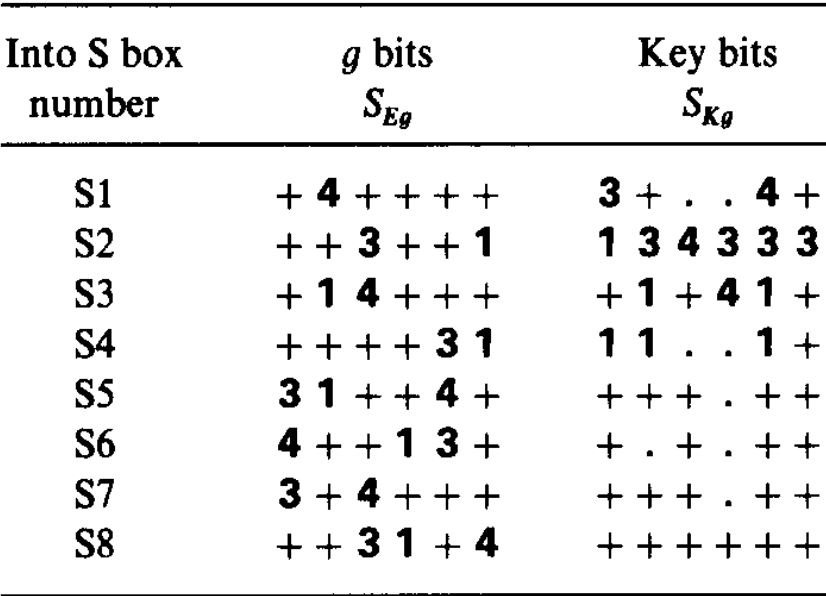
\includegraphics[width=0.5\linewidth]{images/des_8round_dep.png}
    \caption{Dependence of bits at the seventh round on those of the eighth round. `+' indicates dependence on known key bits, `.' indicates dependence on other key bits and a number indicates dependence on unknown key bits that enter the corresponding S box in the eighth round.}
    \label{fig:des-8rd-dep}
\end{figure}

\end{document}
